\documentclass[a4paper]{mwart}

% PACKAGES
\usepackage[utf8]{inputenc}
% \usepackage{fontspec}
\usepackage[T1]{fontenc}
\usepackage{float}
\usepackage{graphicx}
\usepackage{listings}
\usepackage{gensymb}
\usepackage{xcolor}
\usepackage{hyperref}
\hypersetup{%
  colorlinks=true,
  linkcolor=blue,
}

\title{Gliwice360 \\ Aplikcja do zwiedzania Gliwic \\ \url{https://gliwice360.xyz}}
\author{Szymon Hankus}
\date{\today}
% Aby skasować datę, można wstawić \date{} (z pustymi parametrami)

\begin{document}
\maketitle
\begin{figure}[H]
\centering
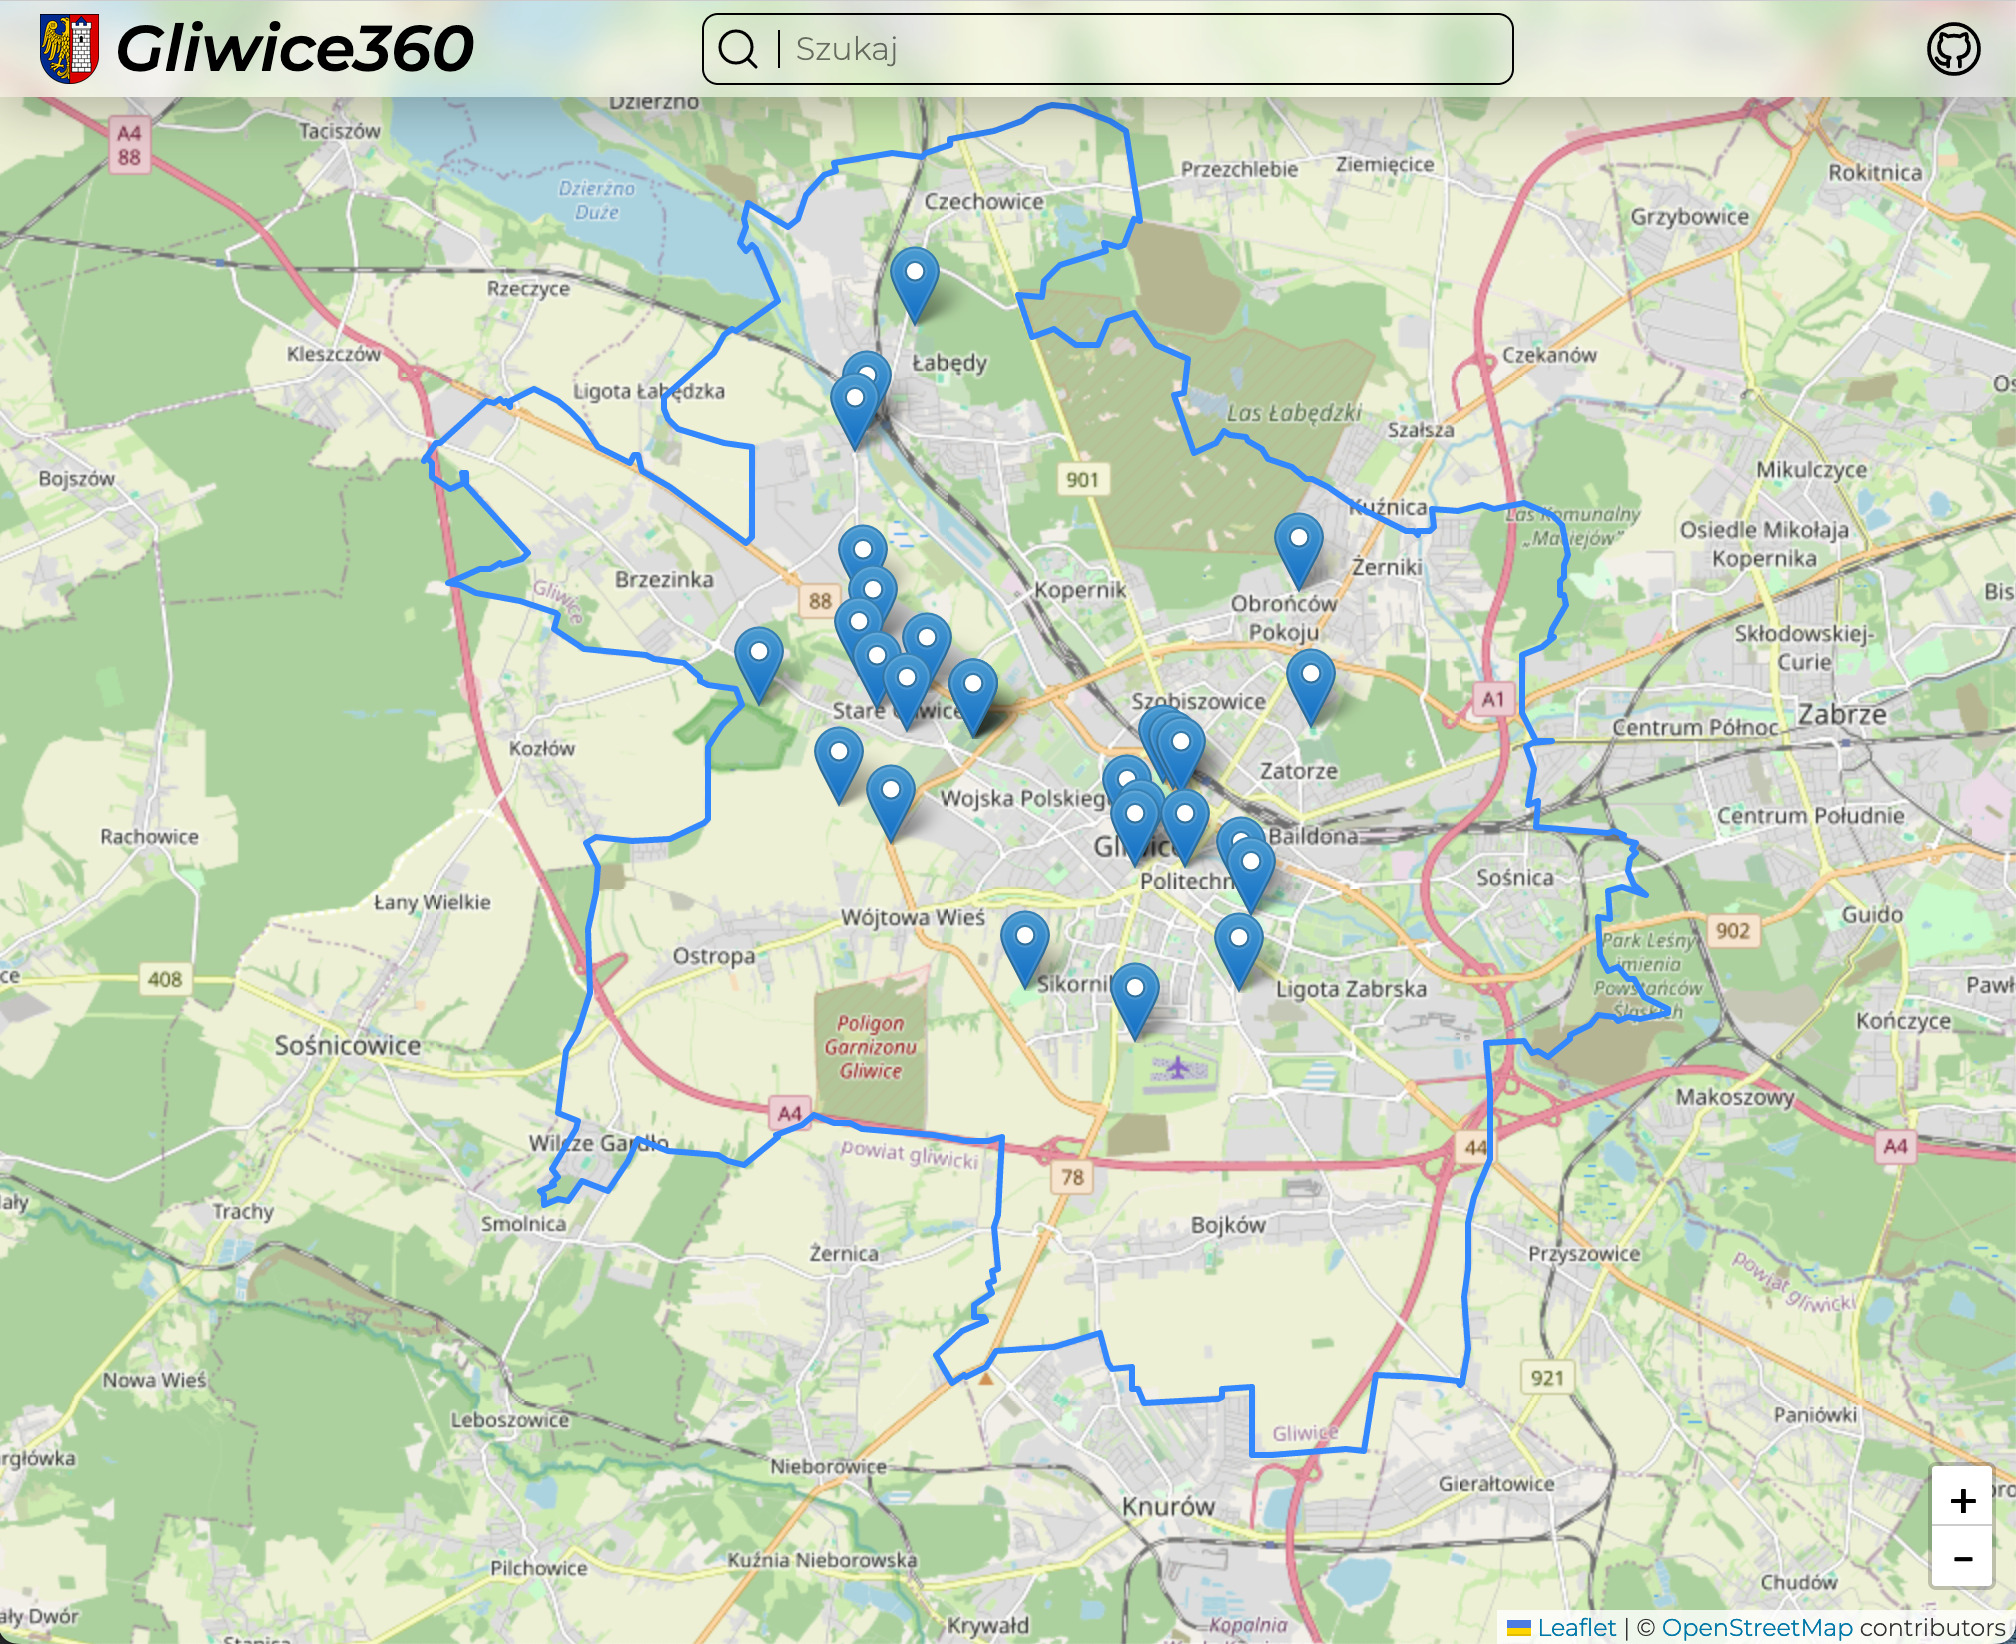
\includegraphics[width=\textwidth]{images/main.jpg}
\end{figure}
\tableofcontents
\newpage

\section{Wstęp}
Ten dokument ma na celu przedstawienie problemu projektowego wraz z jego
rozwiązaniem. Projekt został przygotowany jako jeden z elementów potrzebnych do
zaliczenia przedmiotu ,,Fotografia cyfrowa'' prowadzonego przez doktora Piotra
Gawrona.

\subsection{Motywacja}
Celem projektu było oczywiście wykonanie estetycznych zdjęć, lecz miały być one
częścią jakiegoś głębszego pomysłu. Po ostatnich (moich pierwszych) wyborach
samorządowych zacząłem interesować się sprawami lokalnymi i doceniać wartość 
samorządu, a także wkładu, który każdy może w nim mieć. Mój pomysł -- aplikacja
z panoramami sferycznymi różnych miejsc w Gliwicach umiejscowionych na mapie --
jest więc wyrazem lokalnego patriotyzmu do mojego rodzinnego miasta.

\section{Pomysł i realizacja}
Moim pomysłem było wykonanie wielu panoram sferycznych w różnych zakątkach
Gliwic, a następnie udostępnienie na stronie internetowej w formie interaktywnej
-- mapy z punktami orientacyjnymi, które po kliknięciu prowadzą do przeglądarki
panoram sferycznych, podobnie jak w Google StreetView.

\subsection{Narzędzia}
Do projektu postanowiłem wykorzystać aparat \textit{CANON EOS 200D} oraz
obiektyw typu fish-eye \textit{Sigma 8mm 1:3.5 EXDG}. Aparat umieszczałem na 
monopodzie (statywie jednonożnym) przy pomocy głowicy
\textit{Novoflex OPL VR-SLANT}, a następnie robiłem 4 zdjęcia obracając się w 
osi pionowej o 90 stopni co każde zdjęcie. Taki sposób pozwala na uzyskanie
pełnej panoramy sferycznej 180\degree \(\times \) 360\degree.

\subsection{Oprogramowanie}
Stronę internetową postanowiłem przygotować przy użyciu cenionego obecnie
frameworku \textit{React}, a także bibliotek przygotowanych przez społeczność
open-source. Wykorzystałem 2 główne biblioteki: 
\begin{enumerate}
    \item Leaflet -- integracja z otwartymi mapami społecznościowymi -- \textit{OpenStreetMap}
    \item Photo-sphere-browser -- przeglądarka panoram sferycznych
\end{enumerate}

Do składania zdjęć z aparatu w panoramy wykorzystałem otwartoźródłowy program
\textit{Hugin}.


\section{Rezultat}
Udało mi się stworzyć stronę internetową udostępnianą po protokole HTTPS na
serwerze Nginx z certyfikatem uzyskanym przez platformę \textit{Let's Encrypt}. 
Interfejs strony prezentuje się następująco:
\begin{figure}[H]
\centering
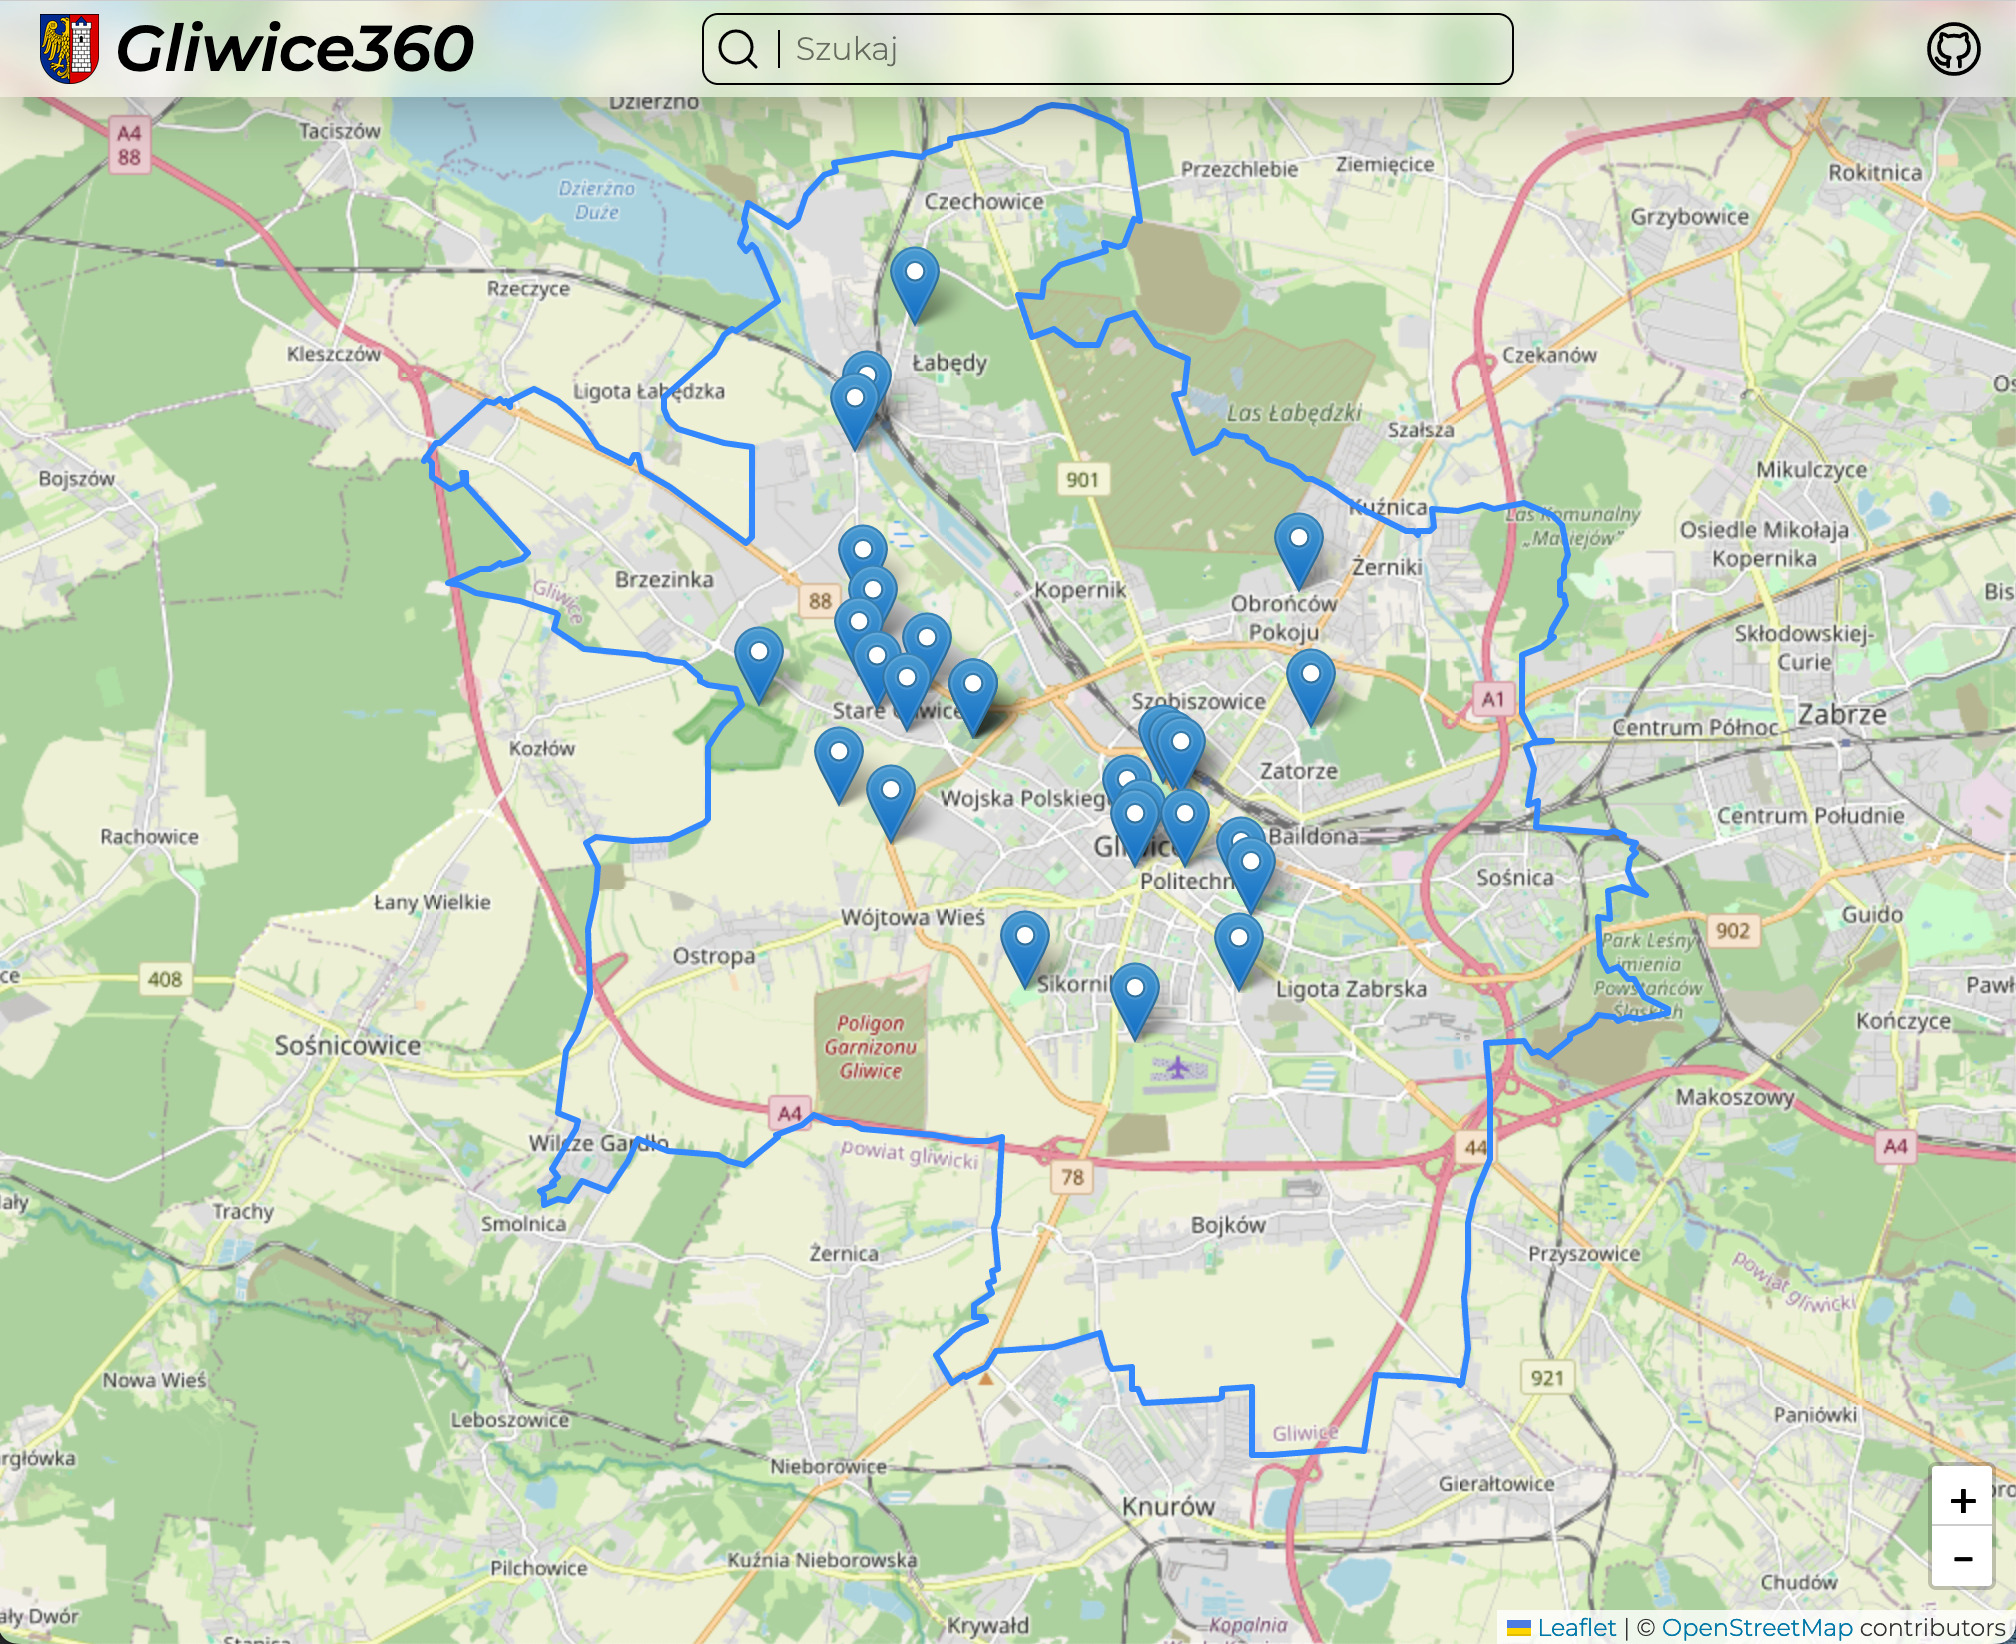
\includegraphics[width=0.9\textwidth]{images/main.jpg}
\end{figure}

Każdy punkt jest oznaczony niebieską ikonką ,,pinezki'' , która wyświetla
podgląd panoramy
sferycznej po najechaniu myszką.
\begin{figure}[H]
\centering
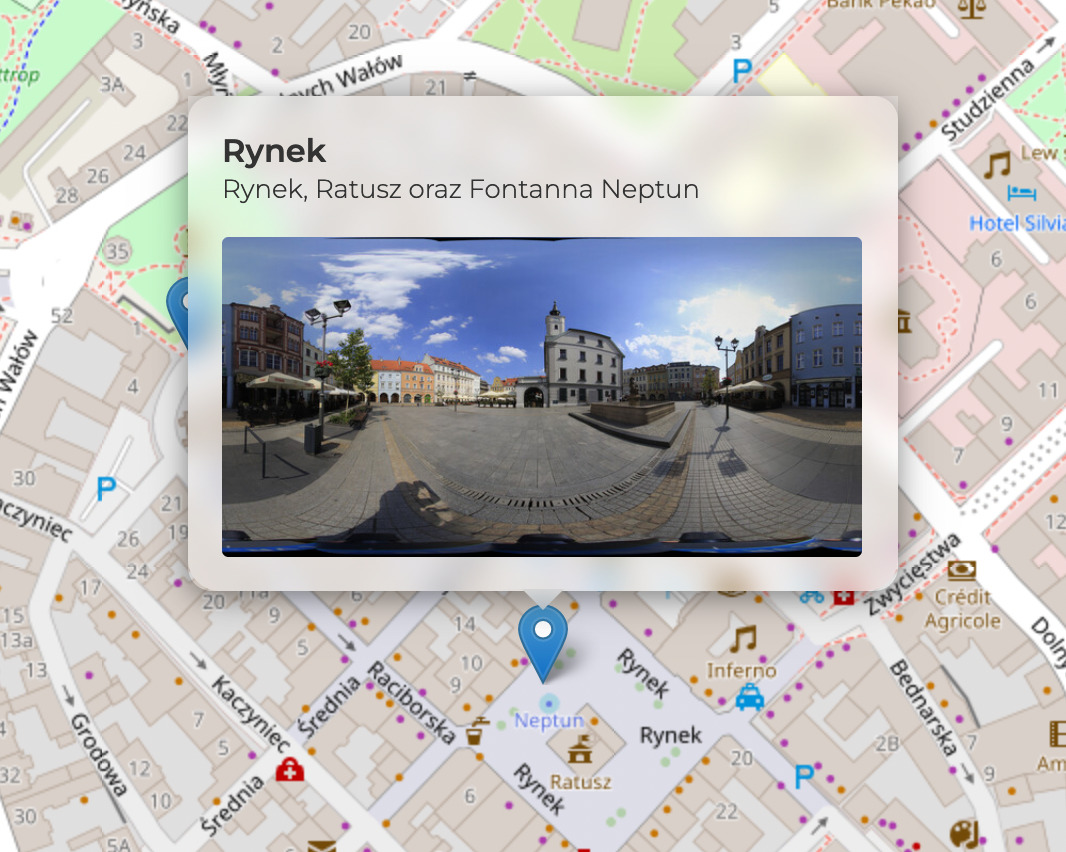
\includegraphics[width=0.9\textwidth]{images/hover.jpg}
\end{figure}

Aby przejść do przeglądarki danej panoramy, należy kliknąć w odpowiadający jej 
punkt.
\begin{figure}[H]
\centering
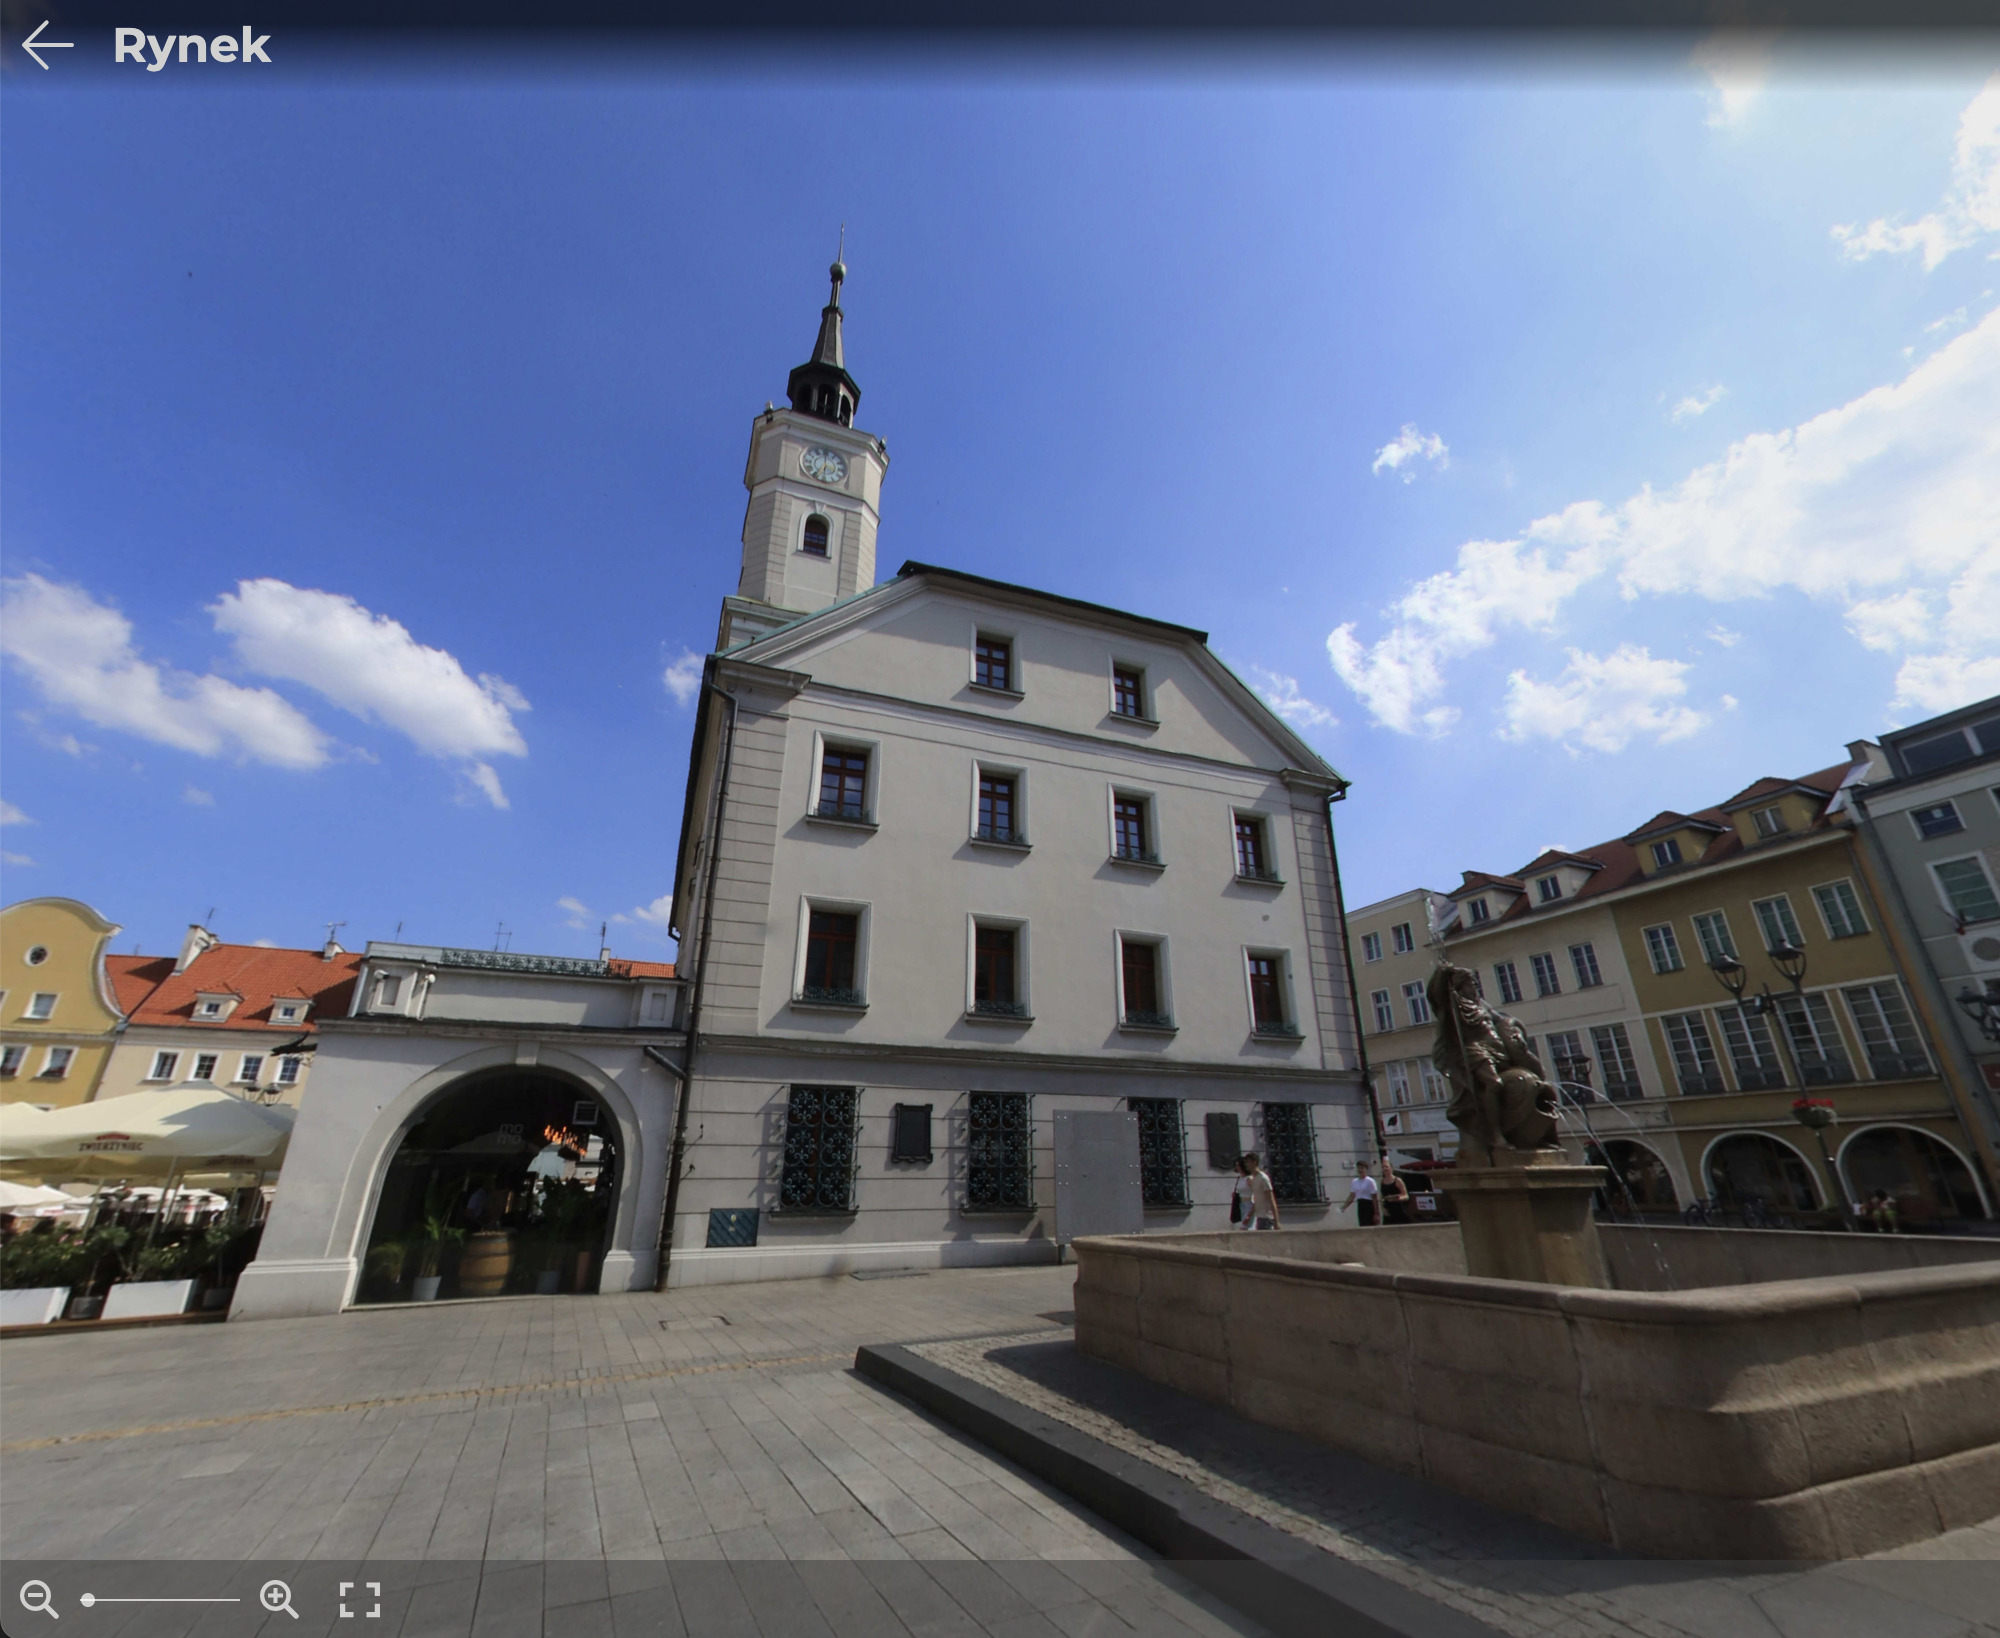
\includegraphics[width=0.9\textwidth]{images/panoview.jpg}
\end{figure}

Punkty możemy też przeglądać i wyszukiwać po kliknięciu w pole \textit{Szukaj}
\begin{figure}[H]
\centering
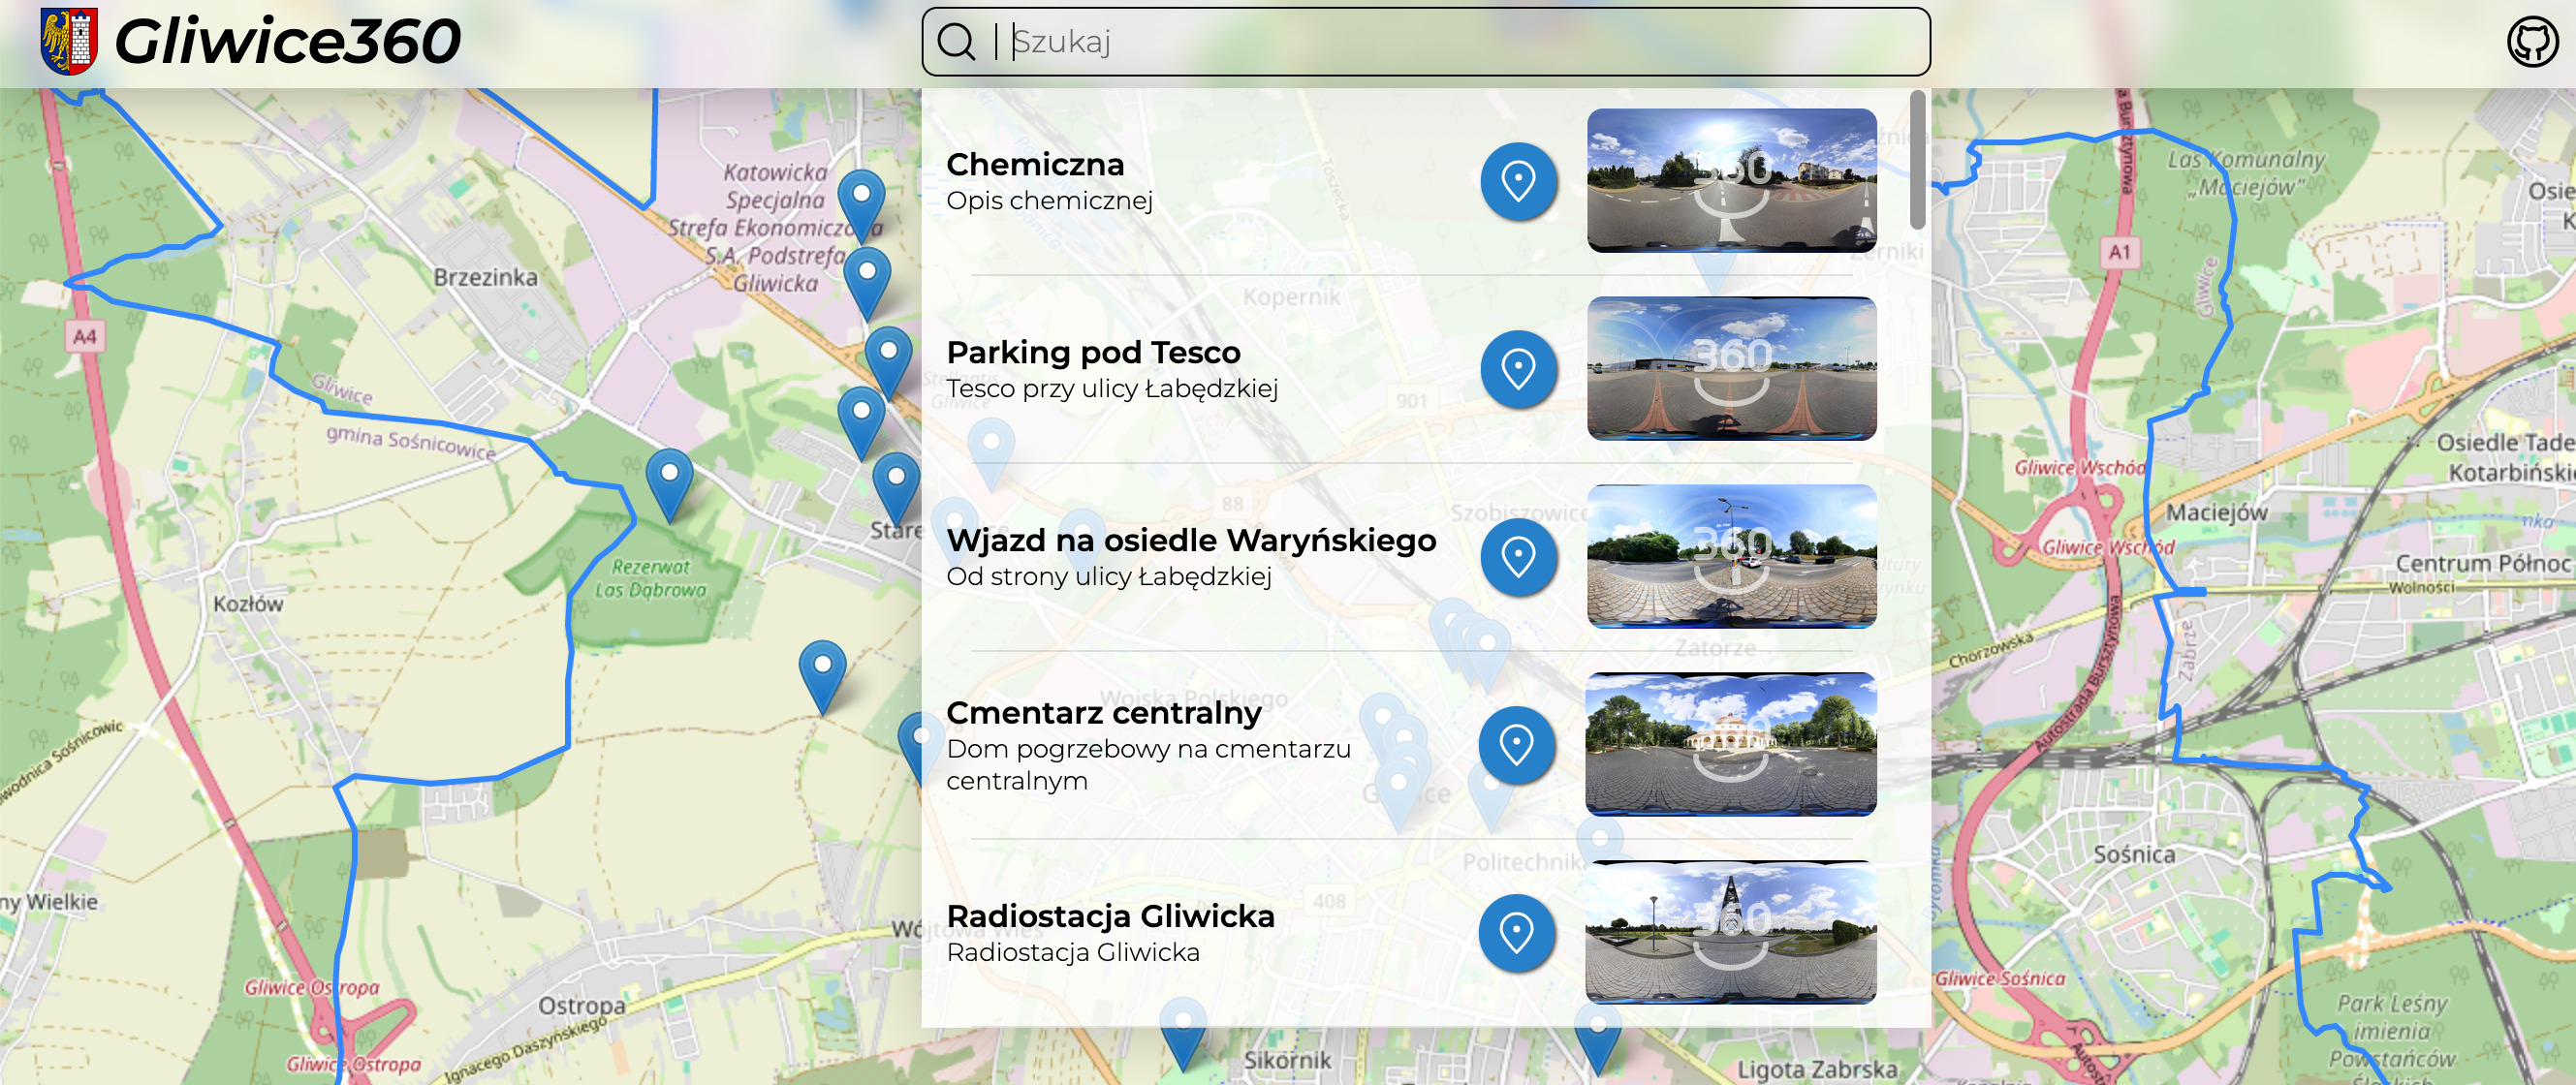
\includegraphics[width=0.9\textwidth]{images/search.jpg}
\end{figure}

Gdy pole wyszukiwania jest puste, domyślnie wyświetlane są wszystkie panoramy,
które możemy przewijać. Można także wpisać dowolny ciąg znaków i znaleźć
panoramę, w której nazwie lub opisie znaduje się tenże ciąg.
\begin{figure}[H]
\centering
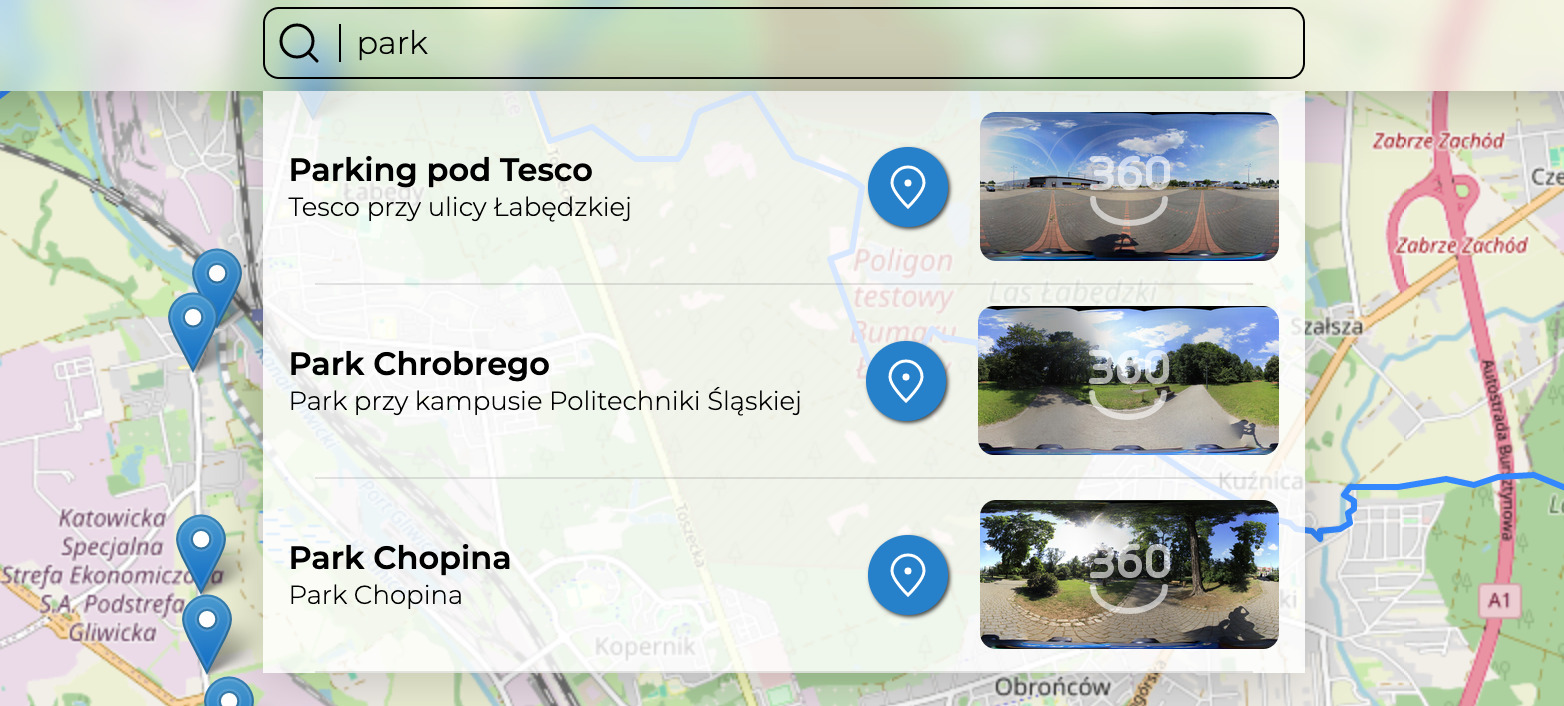
\includegraphics[width=0.9\textwidth]{images/search_query.jpg}
\end{figure}

Aby przejść do punktu na mapie, na mapie należy kliknąć niebieską ikonkę,
natomiast żeby uruchomić przeglądarkę panoramy, należy kliknąć na jej
miniaturowy podgląd.

\section{Napotkane problemy}
Pozwolę sobie pominąć opowieść o napotkanych problemach przy pisaniu kodu
aplikcaji, gdyż dokumentacja stałby się nazbyt techniczna i mało interesująca.
Zamiast tego, skupię się na problemach ze zdjęciami i ich obróbką.

\subsection{Hugin}
Hugin jest programem dla profesjonalistów, co oznacza, że cechuje się wysokim
poziomem skomplikowania. Nauka obsługi tego narzędzia zajęła mi sporo czasu i
sprawiła wiele problemów. Najbardziej poważnym z nich jest problem z
automatycznym znajdowaniem punktów kontrolnych -- miejsc, dzięki którym Hugin
wie jak skleić ze sobą 2 różne zdjęcia. Funkcjonalność ta działał w ok. 60\%
przypadków. Gdy nie podziałała automatyka, trzeba było manualne wybierać punkty
kontrolne (przynajmniej 3-4 na każdą parę zdjęć), co pozwalało usunąć większość
niepożądanych efektów (krzywo sklejonych zdjęć).

\begin{figure}[H]
\centering
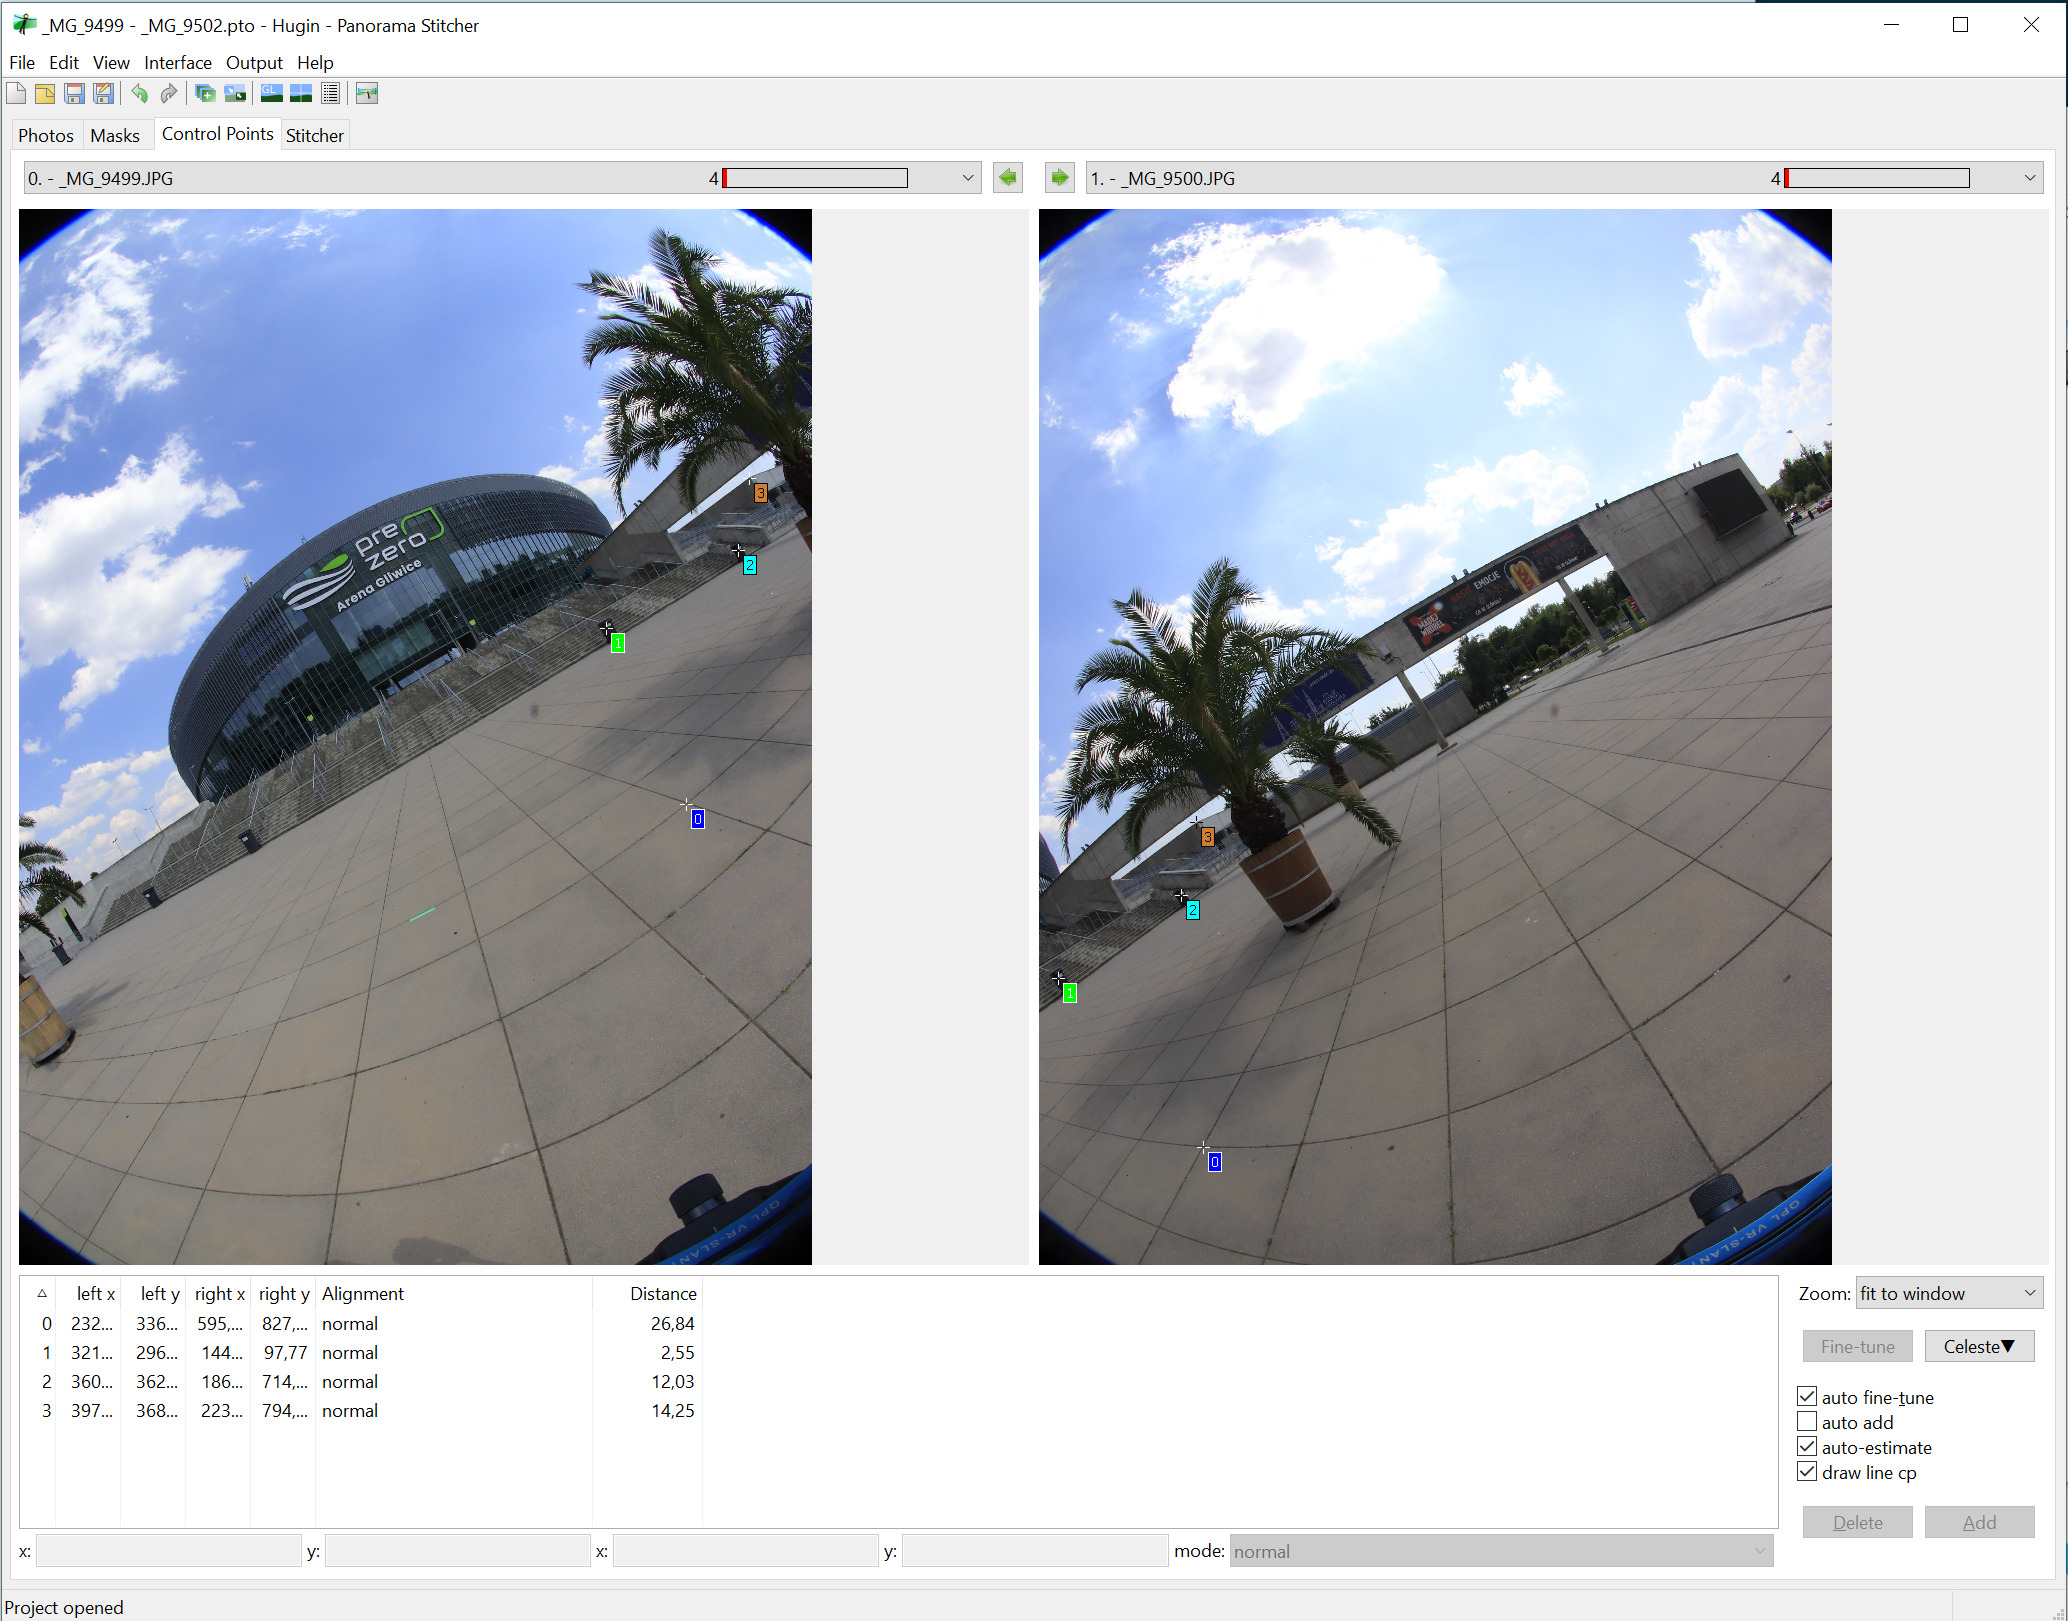
\includegraphics[width=0.9\textwidth]{images/control_points.jpg}
\end{figure}

Niestety na niektórych zdjęciach, mimo ręcznie wybranych punktów kontrolnych,
ostały się nieliczne błędy w sklejanu. Nie udało mi się ich usunąć.
\begin{figure}[H]
\centering
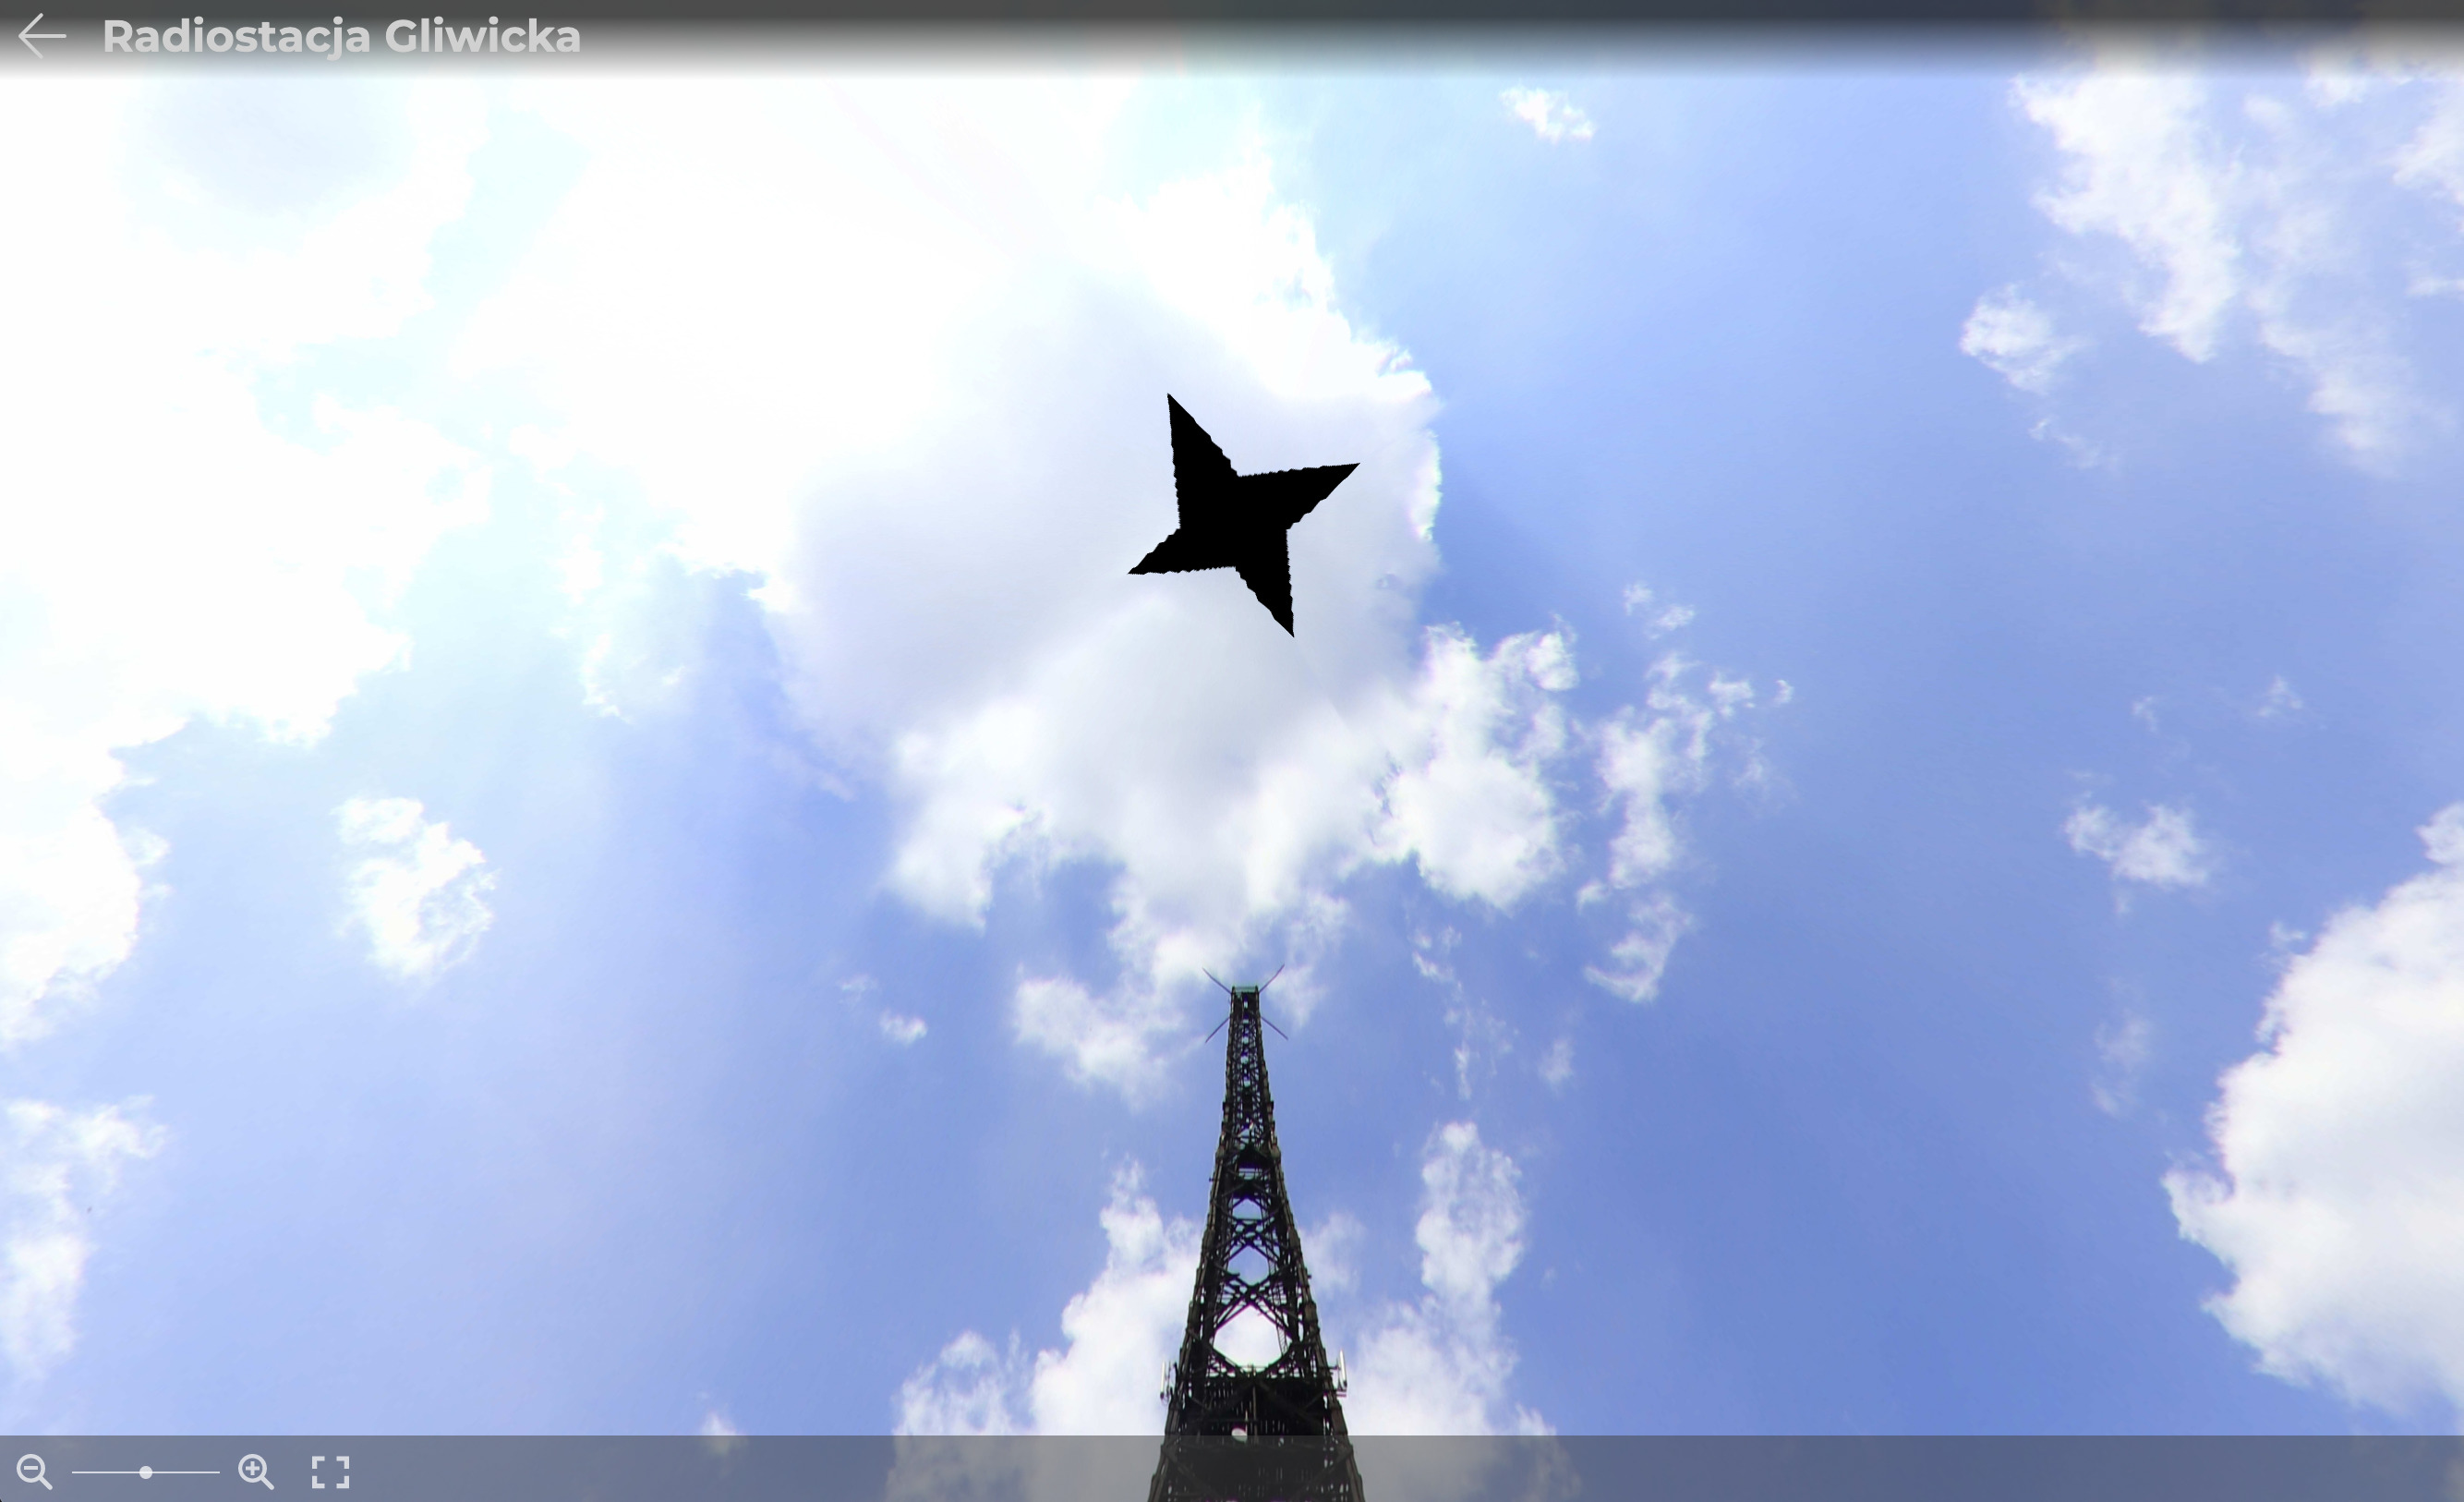
\includegraphics[width=0.9\textwidth]{images/radiostation_error.jpg}
\end{figure}

\subsection{HDR}
Przy robieniu zdjęć pod koronami drzew (np. \textit{Las Dąbrowa}) zorientowałem
się, że aby jaśniejsze i ciemniejsze elementy zdjęcia były jednocześnie wyraźne
potrzebne będą zdjęcia HDR.
\begin{figure}[H]
\centering
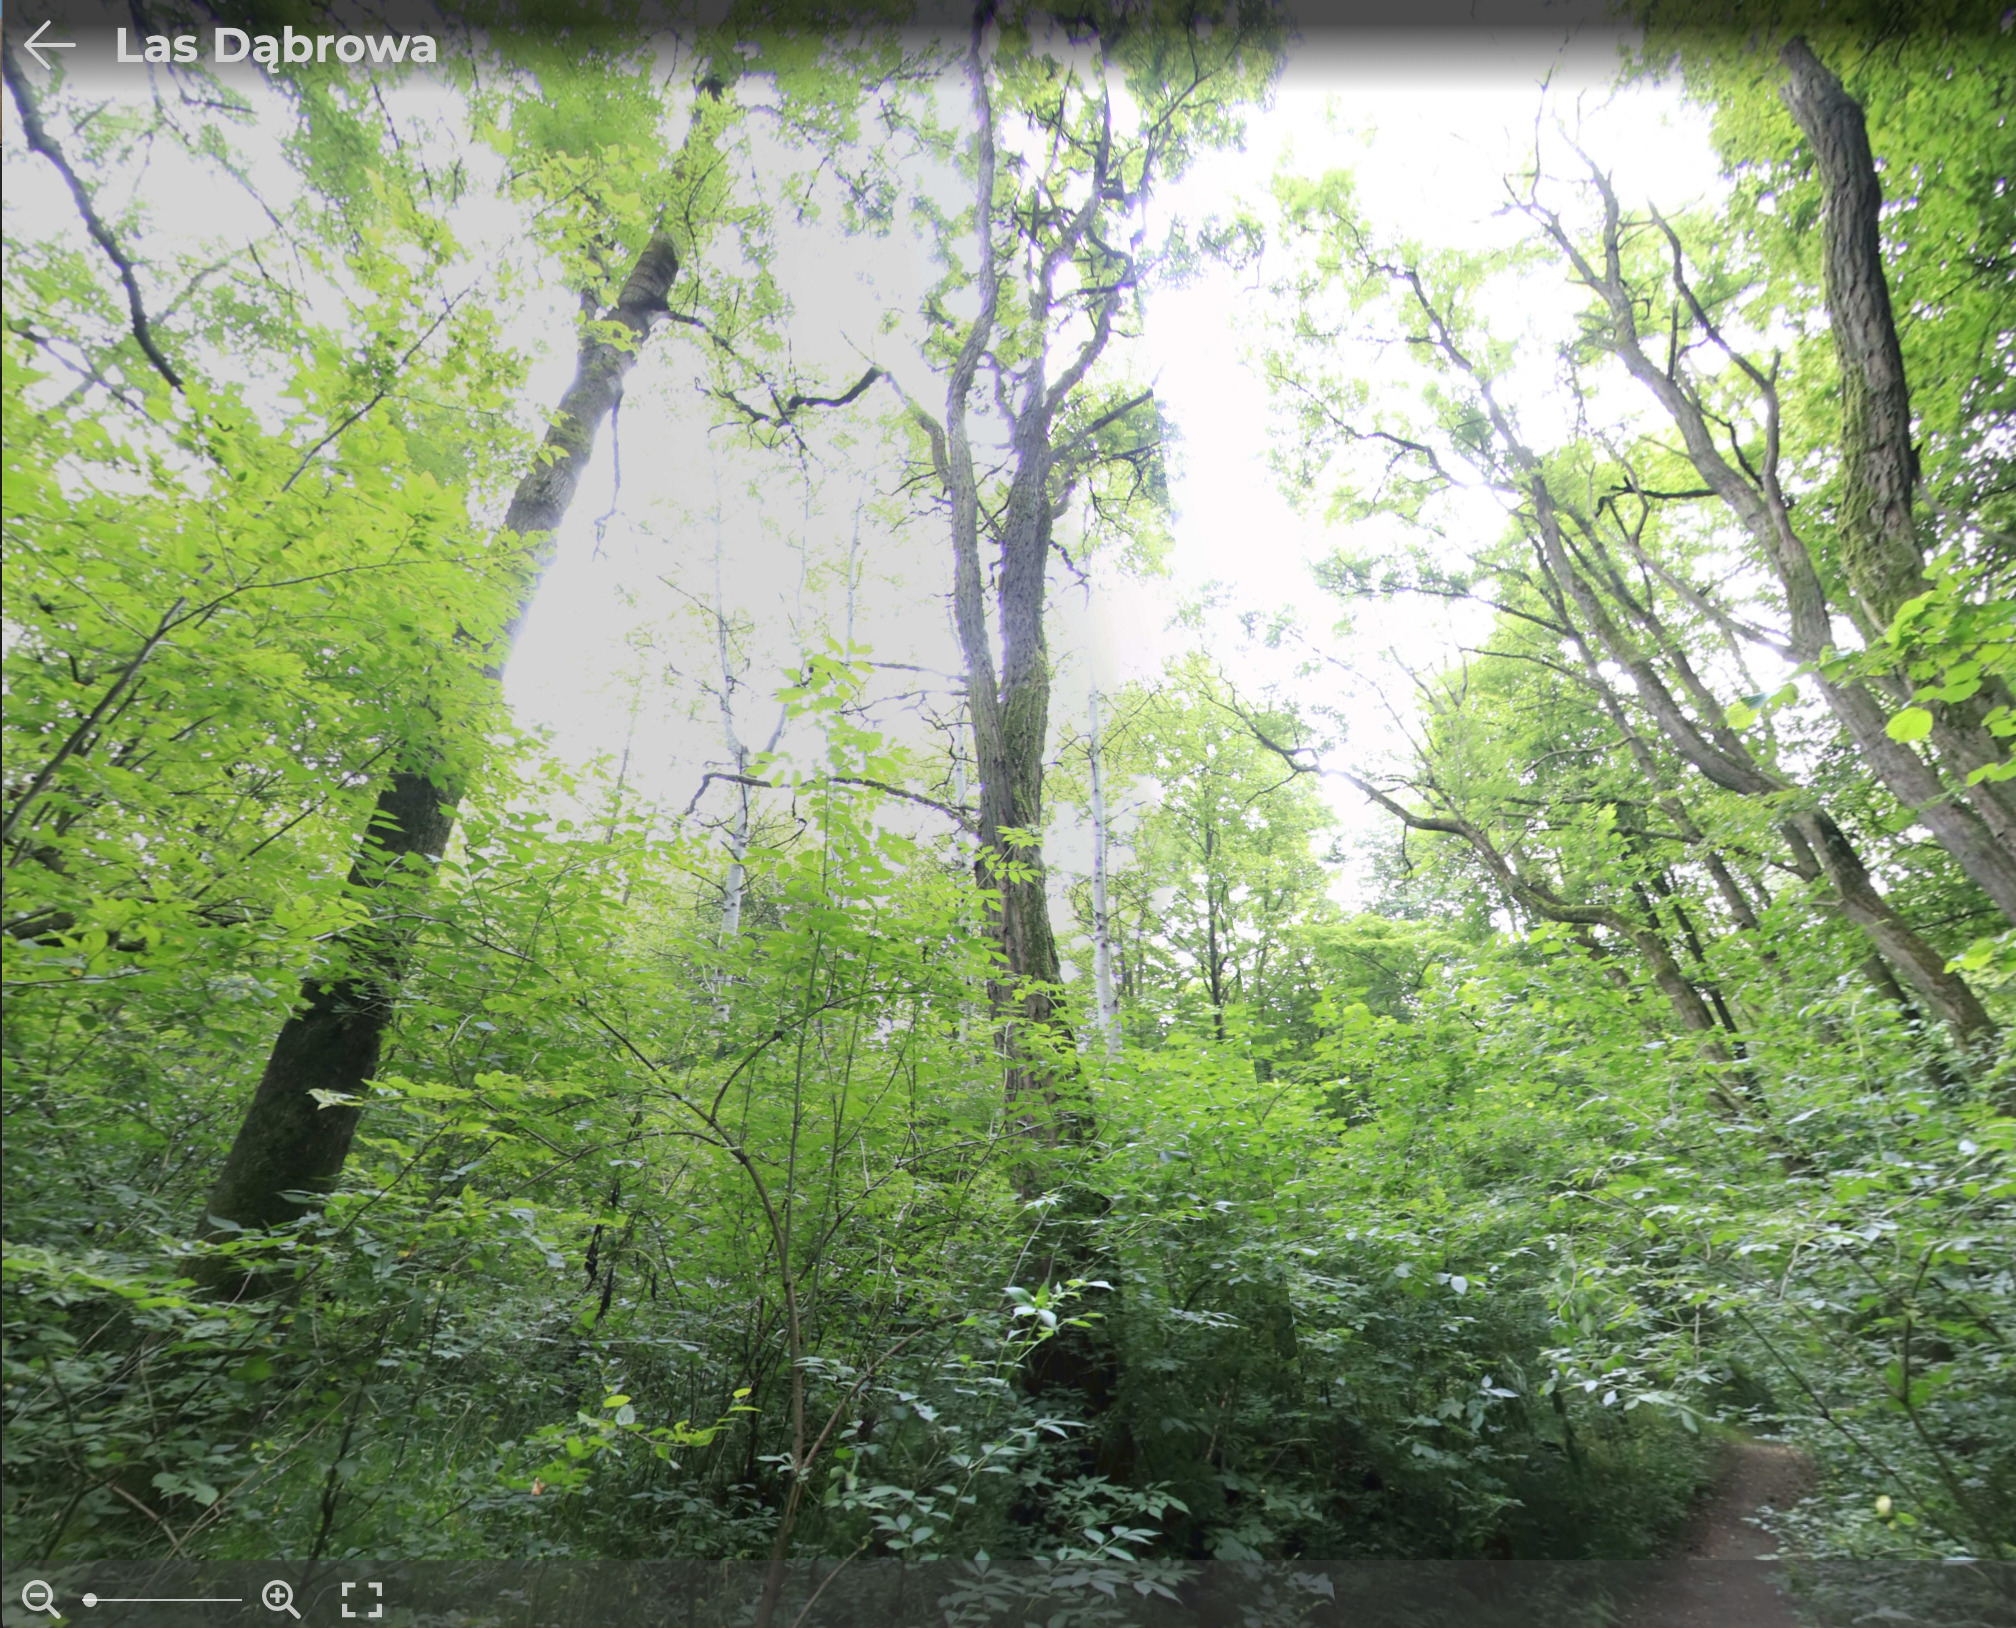
\includegraphics[width=0.9\textwidth]{images/dabrowa.jpg}
\end{figure}

W niektórych panoramach (np. \textit{Cmentarz centralny}) wykorzystałem
funkcjonalność \textit{,,bracketingu''}, co pozwoliło mi na uzyskanie lepszej
kontrastowości jasnych i ciemnych części zdjęcia. 
\begin{figure}[H]
\centering
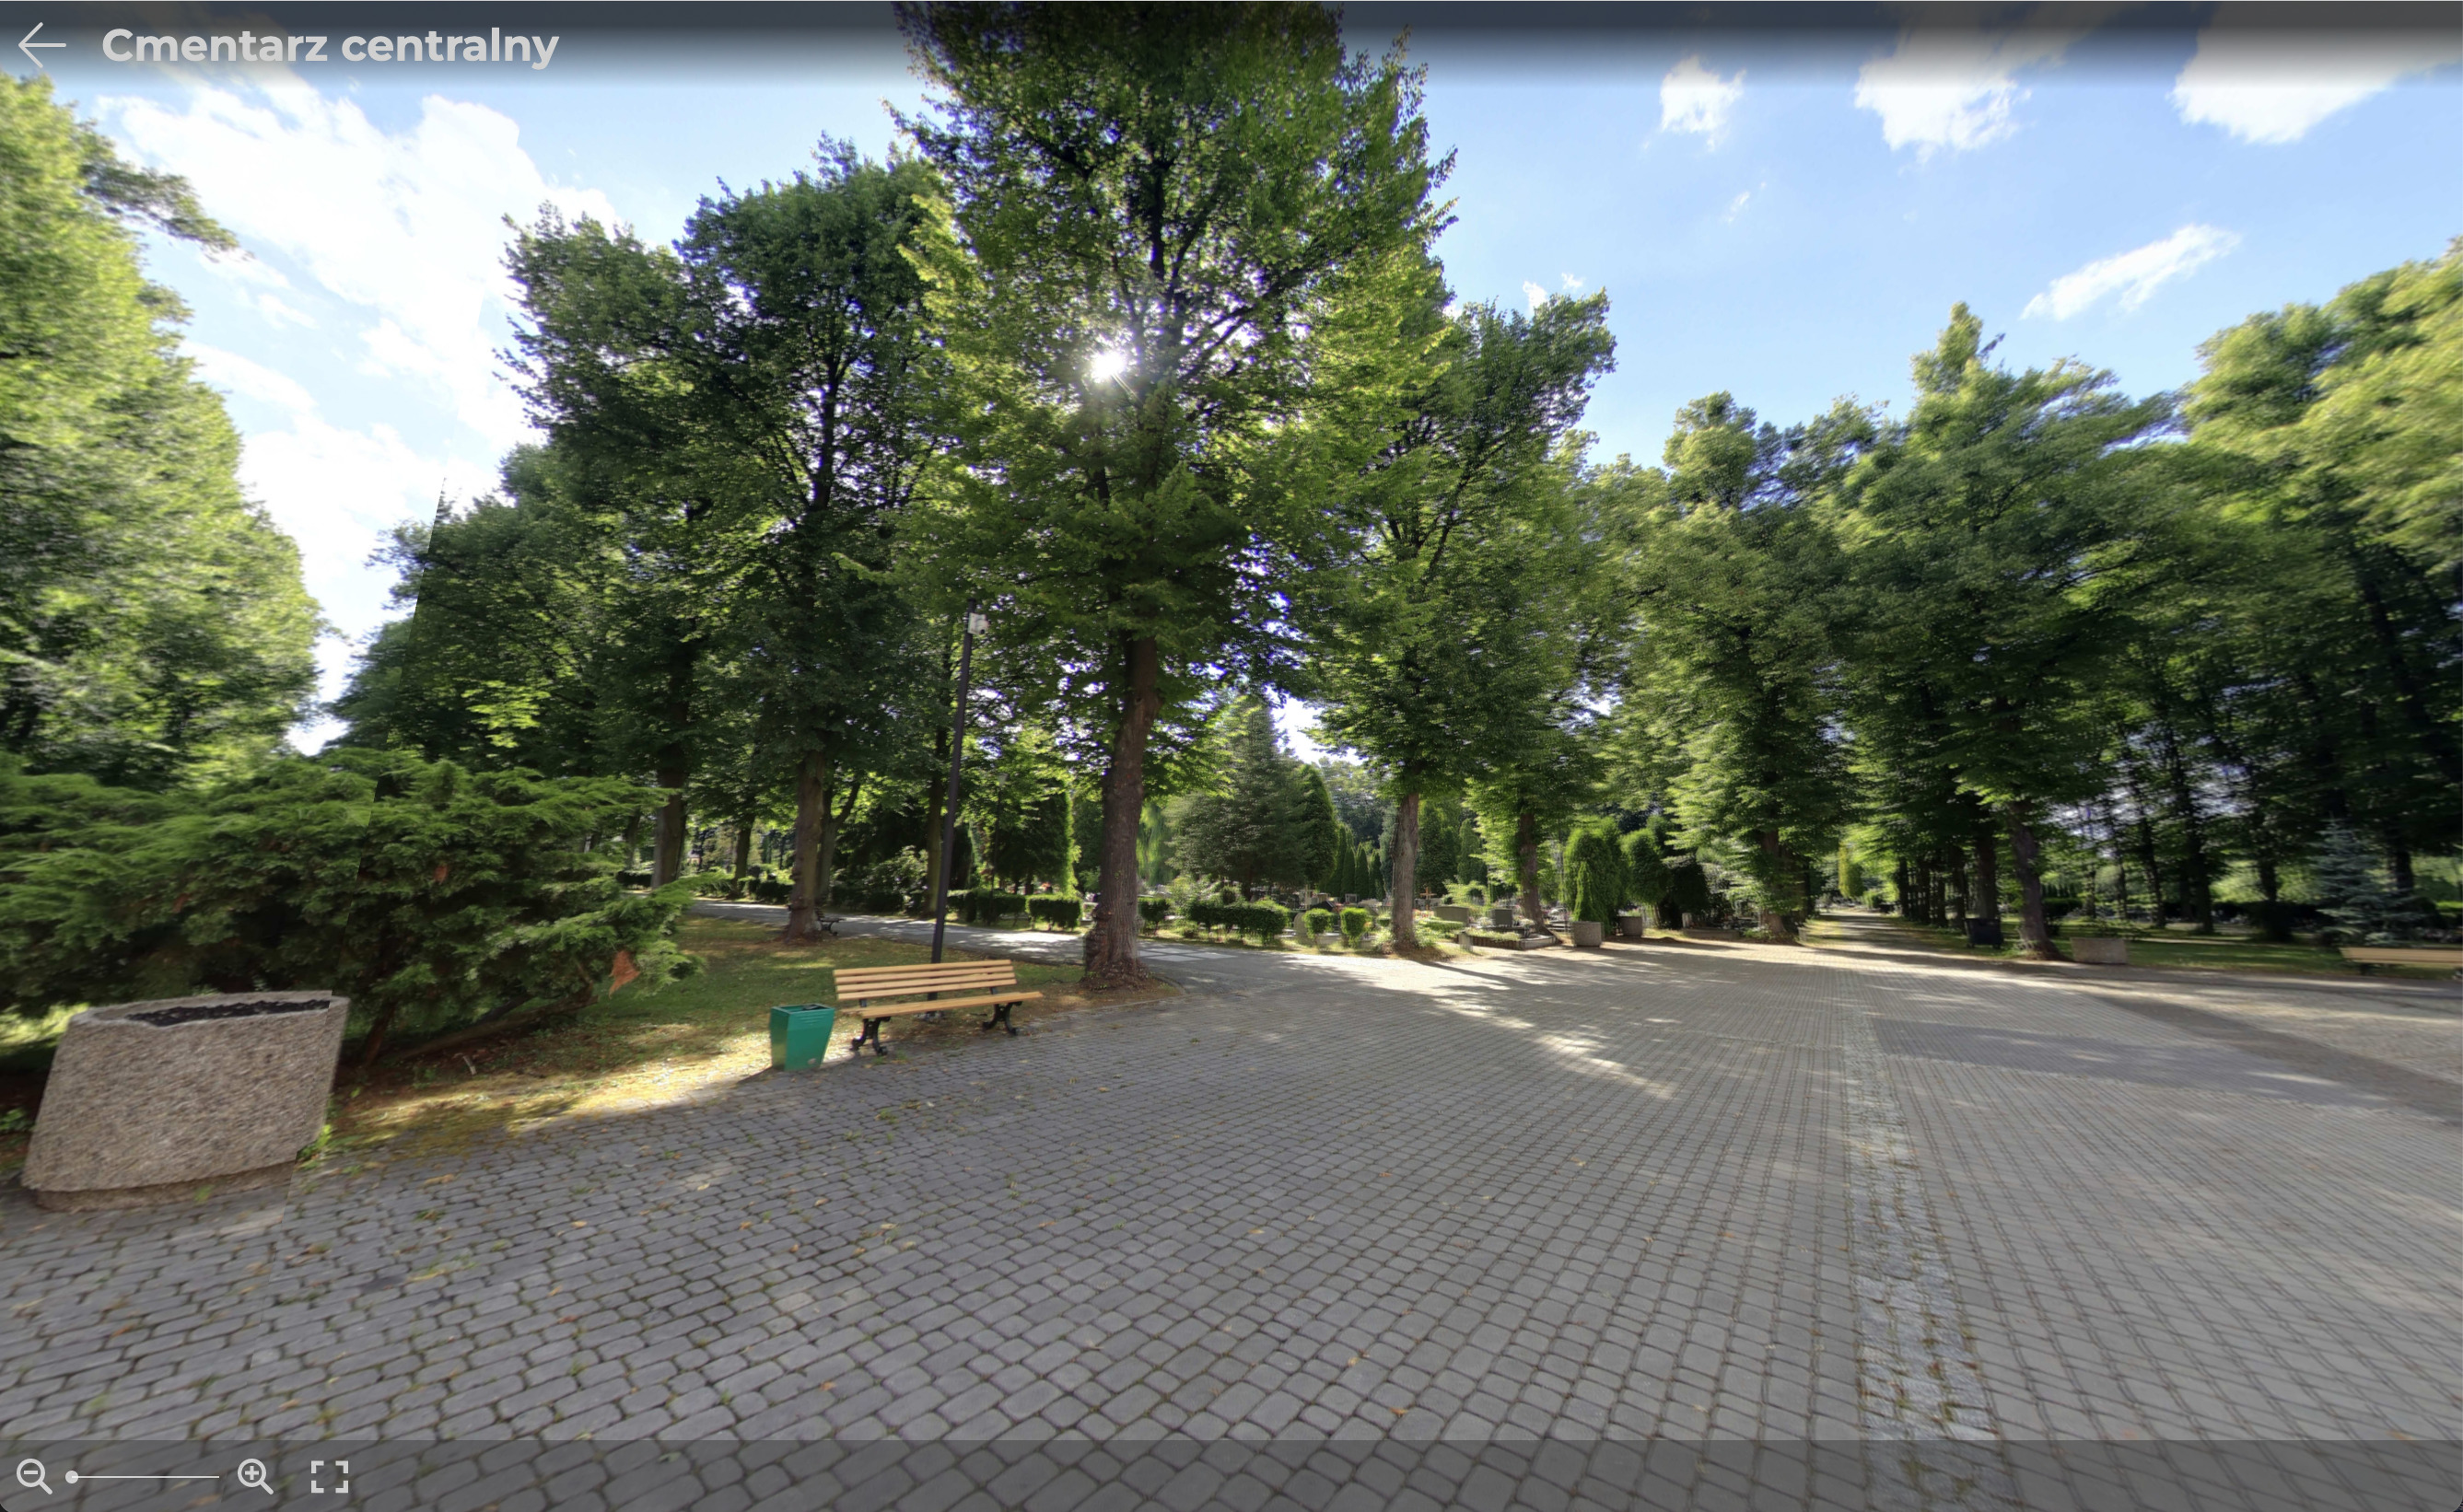
\includegraphics[width=0.9\textwidth]{images/cemetary.jpg}
\end{figure}

\subsection{Rozmiar panoram}
Po sklejeniu panoram okazało się, że wynikowe pliki jpg zajmują niekiedy 20MB,
co jest nieakceptowalne z punktu widzenia użytkownika aplikacji -- w celu
obejrzenia panoramy przeglądarka musi pobrać zdjęcie o rozmiarze kilkunastu
megabajtów, co, w zależności od łącza internetowego, może trwać bardzo długo.
Zdecydowałem się na kompresję zdjęć przy pomocy oprogramowania otwartoźródłowego
ImageMagick, dzięki czemu zdjęcia liczą teraz kilka, a nie kilkanaście
megabajtów.
\begin{figure}[H]
\centering
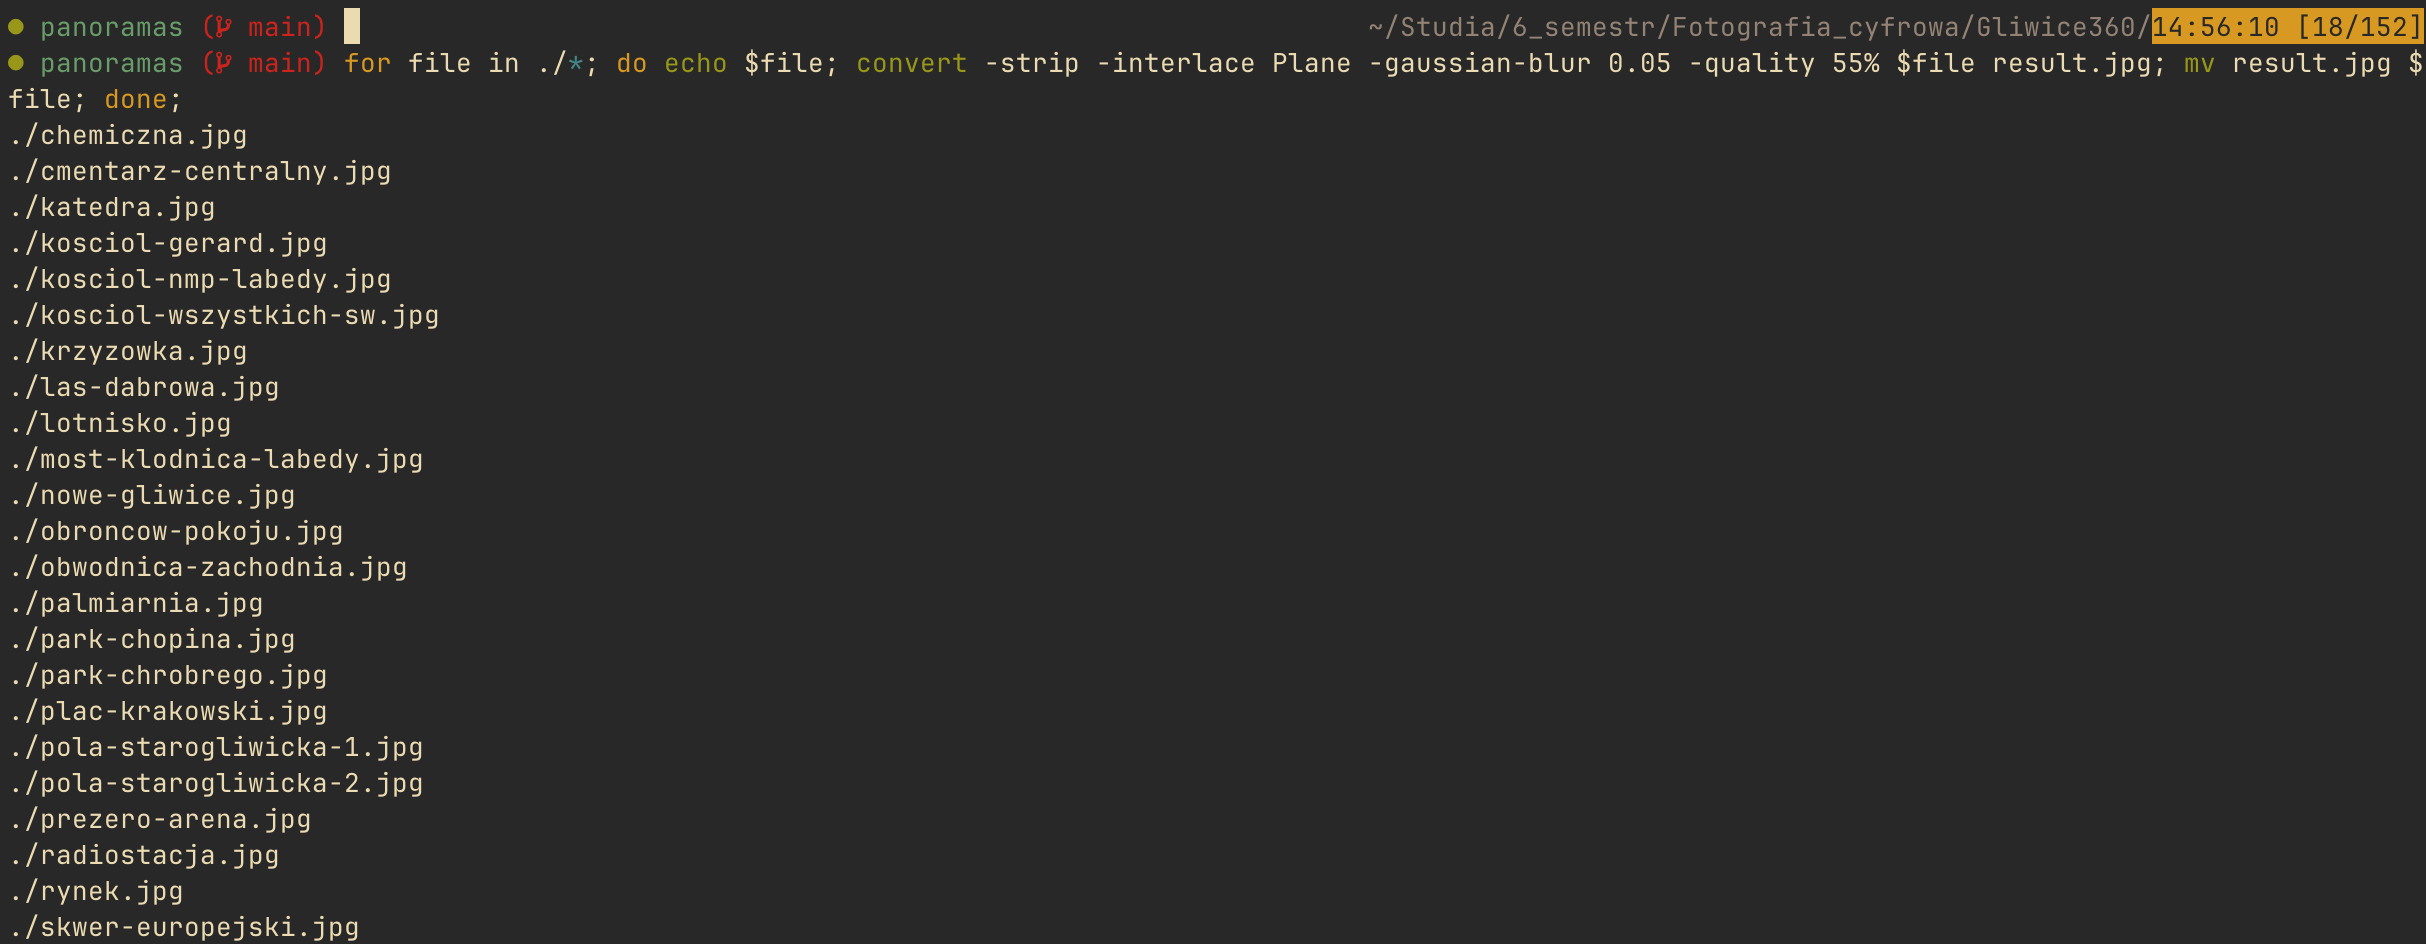
\includegraphics[width=0.9\textwidth]{images/convert.jpg}
\end{figure}

\section{Wnioski}
Projekt zajął mi więcej czasu niż się spodziewałem -- jeżdżenie po Gliwicach 
zarówno rowerem, jak i samochodem jest bardzo czasołchłonne. Procesy składania
panoram, manualnego wybierania punktów kontrolnych, a także pisanie samej
aplikacji nie są czynnościami szybkimi, ani łatwymi. Musiałem nauczyć się
obsługi aparatu, programu Hugin, a także kilku bibliotek JavaScript.
Wynik końcowy mówi jednak sam za siebie i uważam, że warto było podjąć się tego
wyzwania.

\end{document}
